\documentclass[12pt]{article}
\usepackage[utf8]{inputenc}
\usepackage[margin=1in]{geometry}
\usepackage{tikz}
\usepackage[hidelinks]{hyperref}

\title{Week 8 Notes}
\author{Dylan Ang}
\date{May 2021}

\begin{document}

\maketitle

\tableofcontents

\section{Mutualism, Conditional Interactions, Succession}

\begin{table}[h]
    \centering
    \begin{tabular}{c |c | c | c|}
          & -                    & 0                         & +                         \\ \hline
        - & Competition          & Amensalism                & Predation                 \\\hline
        0 & Amensalism           & No Interaction            & Commensalism Facilitation \\\hline
        + & Predation Parasitism & Commensalism Facilitation & Mutualism                 \\\hline
    \end{tabular}
\end{table}

Symbolism: An interaction between two species living in close association with each other (does not necessarily have to be a positive interaction

\subsection{Facilitation}
\begin{itemize}
    \item An interaction in which the presence of one species alters the environment in a way that enhances growth, survival or reproduction of a second, neighboring species.
    \item Example: Limber Pine trees provide shade for young Douglas Fir trees. Shade has a positive impact on Douglas Fir survival because UV rays can be damaging.
\end{itemize}

\subsection{Obligate Mutualism}
\begin{itemize}
    \item Individuals are obligated to participate in the relationship. Species can not function or survive without relationship.
    \item Example: Yucca glauca and Yucca moth. The Yucca plant is only pollinated by the Yucca moth, and the moth reproduces within the flowers of the plant. Yucca moth lays eggs in the plant such that larvae will be within the fruit of the plant.
    \item Costs and benefits
          \begin{itemize}
              \item Yucca Plant: gets flowers pollinated, able to produce fruit. But, the larvae may harm the fruit.
              \item Yucca moth: Fruit provide sustenance for larvae.
              \item If the moth leaves too many larvae, the plant will abort development of that flower.
          \end{itemize}
\end{itemize}

\subsection{Facilitative Mutualism}
\begin{itemize}
    \item A type of mutualism in which the interacting species derive benefit from each other but not being fully dependent that each cannot survive without the symbiotic partner.
    \item Plants and Mycorrhizae: Plants and Fungi can survive without the relationship, but do better together.
\end{itemize}

\subsection{Conditional Interactions}
\begin{itemize}
    \item Occur when the status of the interaction depends on the environment.
    \item Example: Plants and Mycorrhizae. If Nutrient/water availability is high, plant does not require mycorrhizae, but is still providing sugar.
    \item Example: Mutualistic relationships are more common at higher elevation. Surviving in a high elevation environment is difficult, and individuals require more help.
\end{itemize}

\subsection{Species Interactions and Succession}

\begin{itemize}
    \item Primary vs Secondary Succession
    \item Primary: Total habitat destruction. Starting from bare rock.
          \begin{itemize}
              \item Stages
                    \begin{itemize}
                        \item Bare rock
                        \item Lichens
                        \item Small Plants
                        \item Grasses
                        \item Grasses, shrubs, shade intolerant trees
                        \item Large trees
                    \end{itemize}
          \end{itemize}

    \item Secondary: Sever disturbance, but there is still soil.
          \begin{itemize}
              \item Stages
                    \begin{itemize}
                        \item Bare rock
                        \item Lichens
                        \item Small Plants
                        \item Grasses
                        \item Grasses, shrubs, shade intolerant trees
                        \item Large trees
                    \end{itemize}
          \end{itemize}
    \item Succession may affect a species' realized niche
          \begin{itemize}
              \item A plant that requires a very developed forest system might be around early in a succession environment, but won't operate in that environment until the ecosystem recovers enough to contain the species that they need to interact with.
              \item i.e. Consider a bear. They would likely not return to a succession environment until the environment contains the specie sit relies on: salmon for food, bees to make honey, and large trees to scratch their backs.
          \end{itemize}
\end{itemize}

\section{Biomes}

\begin{itemize}
    \item Biomes are defined by 4 main components
          \begin{itemize}
              \item Average annual temperature
              \item Annual Precipitation
              \item Seasonality: Difference between dry and wet season, and warm and cool season.
              \item Disturbance: How disturbances (fire) affect
          \end{itemize}
\end{itemize}

\subsection{Types of terrestrial biomes}

\begin{figure}
    \centering
    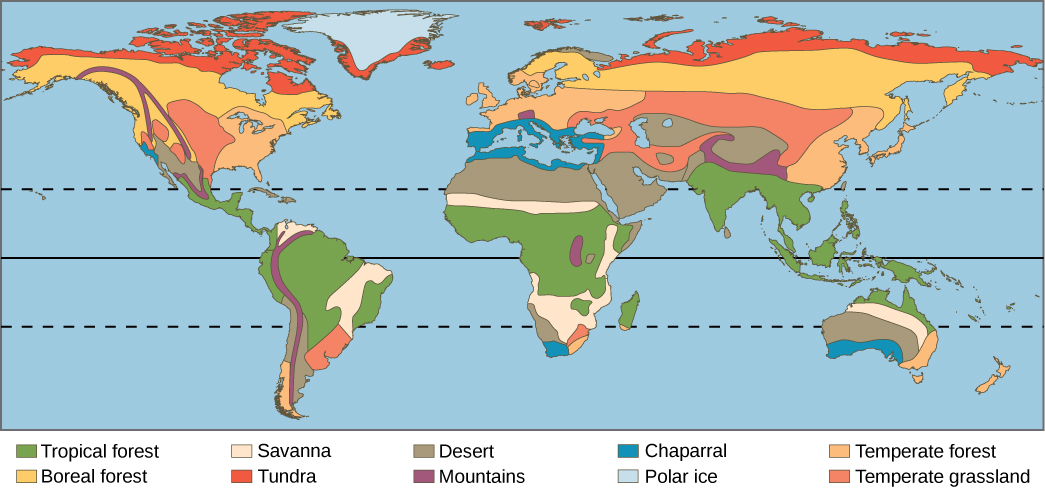
\includegraphics[width=\linewidth]{map.jpg}
    \caption{Locations of Biomes}
\end{figure}

\begin{itemize}
    \item Tropical Rainforest
          \begin{itemize}
              \item High Biodiversity
              \item High precipitation and temperature all year
          \end{itemize}
    \item Temperate Deciduous Forest
          \begin{itemize}
              \item Seasonality in temperature and precipitation
          \end{itemize}
    \item Deserts
          \begin{itemize}
              \item Low Precipitation and High temperature
              \item Temperature has high seasonality
              \item By definition, very dry, but can be cold
              \item Cold desserts can have similar climate graph to Tundra
          \end{itemize}
    \item Tundra
          \begin{itemize}
              \item Seasonality in temperature and extremely low precipitation
              \item Must be high latitude
          \end{itemize}
    \item Boreal Forest - Taiga
          \begin{itemize}
              \item Seasonality in temperature and precipitation
              \item Only in northern hemisphere because the latitude negative is ocean
              \item Low temperatures
          \end{itemize}
    \item Temperate Grassland
          \begin{itemize}
              \item Seasonality in temperature
              \item Slight Seasonality in Precipitation
          \end{itemize}
    \item Mediterranean - Chaparral
          \begin{itemize}
              \item Seasonality in Temperature and Precipitation but they are opposites.
              \item All other biomes have hot wet summers and cold dry summers, Chaparrals have hot dry summers and cold wet winters.
          \end{itemize}
\end{itemize}

\subsection{Aquatic Biomes}

Abiotic conditions that define aquatic biomes.
\begin{itemize}
    \item Salt Content
          \begin{itemize}
              \item Fresh water (Lakes, rivers, streams)
              \item Salt water
              \item Brackish - meh
          \end{itemize}
    \item Pelagic Zones (Ocean Zones)
\end{itemize}

\subsubsection{Wetlands}

\begin{itemize}
    \item Wetland ecosystem services
          \begin{itemize}
              \item Filter pollutants out of the water
              \item Reduce sediment load
              \item Habitat for species (water fowl during breeding)
              \item Absorb storm surges and prevent floods
          \end{itemize}
\end{itemize}

\section{Fire}

\begin{itemize}
    \item Types of Fires
          \begin{itemize}
              \item Ground Fire: Matter below the soil surface.
              \item Surface Fire: Dead or dry vegetation on the ground.
              \item Crown Fire: Burn through the tree canopy. They are very destructive and spread quickly.
          \end{itemize}
    \item Fire adaptations
          \begin{itemize}
              \item Fire tolerators (trees)
                    \begin{itemize}
                        \item Tall with thick bark, no branches near the ground, long needles
                    \end{itemize}
              \item Fire embracers (trees)
                    \begin{itemize}
                        \item Short, thin bark, flammable needles, keep low branches, closed clones
                        \item Cones don't open until experiencing fire
                    \end{itemize}
              \item Fire recruiters (shrubs)
                    \begin{itemize}
                        \item Seeds are dormant until fire, germinate immediately after fire event.
                    \end{itemize}
              \item Fire Persisters (shrubs)
                    \begin{itemize}
                        \item Can resprout from below-ground tissue, no seed dormancy and no adaptations for surviving fire events.
                        \item Essentially just die and hope theres enough time to come back before the next fire.
                    \end{itemize}
          \end{itemize}
    \item Fire Examples
    \begin{itemize}
        \item Prairie fire
        \begin{itemize}
            \item Fire stimulates regrowth of grass
            \item Prevents tree encroachment
            \item Konza Prairie Fire Study
            \begin{itemize}
                \item A plot burned every year is entirely grass
                \item A plot burned every 4 years will have some shrubs
                \item Shrubs protect trees
                \item Trees in areas with more grazing are more resistant to fire because they have less low hanging brush.
            \end{itemize} 
        \end{itemize} 
    \end{itemize} 
\end{itemize}

\end{document}